\documentclass{aip-cp}

\usepackage[numbers]{natbib}
\usepackage{rotating}
\usepackage{graphicx}
\usepackage{enumitem}

%\pdfmapfile{+txfonts.map}

%%%%%������� ��� �������� ������
%\usepackage[utf8x]{inputenc}
%\usepackage[english,russian]{babel}
%\usepackage{cmap}
%%%%%


% Document starts
\begin{document}

% Title portion

\title{A Flexible  Generator of Constrained Global Optimization Test Problems}


\author{Victor Gergel}
\author{Konstantin Barkalov\corref{cor1}}
%\eaddress[url]{http://www.aip.org}
\author{Ilya Lebedev}
%\eaddress{anotherauthor@thisaddress.yyy}
\author{Maria Rachinskaya}
\author{Alexander Sysoyev}

\affil{Lobachevsky State University of Nizhni Novgorod, Nizhni Novgorod, Russia}

\corresp[cor1]{Corresponding author: konstantin.barkalov@itmm.unn.ru}

\maketitle

\begin{abstract}
In the present work, further development of an approach to constructing the test global 
optimization problems with nonlinear constraints is considered. In the generated problems, the 
location of the global minimum is known. The considered generator is featured by an option of 
specifying desired number of constraints and the fraction of feasible domain relative to the 
whole global search domain. In the updated version of the generator, the options of forming the 
problems with a conditional minimum located at the boundary of the feasible domain and of 
specifying the number of constraints active in the minimizer have been added. The 
demonstration of the developed approach is given on the example of a known index method for 
solving the complex multiextremal optimization problems with non-convex constraints.
\end{abstract}

% Head 1
\section{INTRODUCTION}

In the present paper, the methods for generating the global optimization test problems with non-
convex constraints
\begin{eqnarray}
&\varphi(y^\ast)=\min{\left\{\varphi(y):y\in D, \; g_i(y)\leq 0, \; 1 \leq i \leq m\right\}}, 
\label{i_problem} \\
&D=\left\{y\in R^N: a_i\leq y_i \leq b_i, 1\leq i \leq N\right\} \label{D}
\end{eqnarray}
are considered. The objective function $\varphi(y)$ (henceforth denoted by $g_{m+1}(y)$) and 
the left-hand sides $g_i(y), \; 1\leq i \leq m,$ of the constraints are supposed to satisfy the 
Lipschitz condition
\[ \left|g_i(y')-g_i (y'')\right| \leq L_i \left\|y'-y'' \right\|, \; y',y''\in D, \; 1\leq i \leq m+1. \]
with the Lipschitz constants unknown a priori. The analytical formulae of the problem functions 
may be unknown, i.e. these ones may be defined by an algorithm for computing the function 
values in the search domain (so called ``black-box''-functions). It is supposed that even a single 
computing of a problem function value may be a time-consuming operation since it is related to 
the necessity of numerical modeling in the applied problems (see, for example, 
\cite{Menniti2008,Kvasov2015,Modorskii2017}).

The evaluation of efficiency of the developed methods is one of the key problems in the 
optimization theory and applications. Unfortunately, it is difficult to obtain any theoretical 
estimates in many cases. As a result, the comparison of the methods is performed by carrying 
out the computational experiments on solving some test optimization problems in most cases. In 
order to obtain a reliable evaluation of the efficiency of the methods, the sets of test problems 
should be diverse and representative enough. The problem of choice of the test problems has 
been considered in a lot of works (see, for example, 
\cite{Floudas1999,Gaviano2003,Ali2005,Addis2007}). Unfortunately, in many cases, the 
proposed sets contain a small number of test problems, and it is difficult to obtain the problems 
with desired properties. The most important drawback consists of the fact that the constraints 
are absent in the proposed test problems as a rule (or the constraints are relatively simple: linear, 
convex, etc.).

In the present work, further development of the approach to generating the global optimization 
problems with non-convex constraints proposed originally in \cite{Gergel2017} has been 
conducted.
When generating the test problems, the necessary number of constraints and the desired fraction 
of the feasible domain relative to the whole global search domain can be specified. 
At that, the location of the global minimum is known for the generated problems that essentially simplifies 
evaluating the results of the numerical experiments. 
In addition to the specified options, the following functions have been added in the current version of the generator: 

\begin{itemize}
\item The possibility to generate the problems with the conditional minimum point located at the 
boundary of the feasible domain.
\item The possibility to specify the number of constraints active in the optimum point.
\end{itemize}

The above capabilities allow emulating the properties of the applied constrained global 
optimization problems more adequately.


\section{TEST PROBLEM CLASSES}
A well-known approach to investigating and comparing the multiextremal optimization 
algorithms is based on testing these methods by solving a set of problems, chosen randomly 
from some specially designed class. 

A generator for random samples of two-dimensional test functions has been 
described, for example, in \cite{Grishagin1997,Grishagin2015}. %more refs
Another generator (\textit{GKLS generator}) for the functions of arbitrary dimensionality with 
known properties (the number of local minima, the size of their domains of attraction, the global 
minimizer, etc.) has been proposed in \cite{Gaviano2003}.  Application of this generator for 
studying some unconstrained optimization algorithms has been described in \cite{Paulavicius2014,Sergeyev2015}. 

The generator GCGen (Global Constrained optimization problem Generator) which allows to 
generate the test global optimization problems with $m$ constraints has been proposed in \cite{Gergel2017}. In this paper, the rules, which allow formulating the constrained global optimization problems have been proposed so that:
\begin{itemize}
	\item one could control the size of feasible domain with respect to the whole domain of 
the parameters' variation;
	\item the global minimizer of the objective function would be known a priori taking into 
account the constraints;
	\item the global minimizer of the objective function without accounting for the 
constraints would be out of the feasible domain.
\end{itemize}


The location of the conditional minimum at the boundary of the feasible domain is an important 
property featuring the applied constrained optimization problems. 
When generating the problems according to the scheme described in \cite{Gergel2017}, 
the conditional minimum, in general, will be located inside the feasible domain. Therefore, the 
options of shifting the conditional minimum to the boundary of the feasible domain as well of 
specifying the number of the active constraints in this one have been added in the new version 
of the problem generator.

The shifting of the conditional minimum to the boundary of the feasible domain is performed in 
the following way.
\begin{enumerate}
\item A problem with an arbitrary location of the constrained minimum $\overline{y}$ is 
generated;
\item From the point $\overline{y}$, a coordinate search of a feasible point $y^*$, for which at 
least one constraint is active (i.e. there is such index $j, 1 \leq j\leq m$ that $\left|g_j(y^*)\right| 
\leq \delta$) is performed with given step $h$. 
\item A rough estimate of $y^*$ obtained is refined by a local method. 
\item The coordinate transformation transferring the point $\overline{y}$ to the point $y^*$ is 
performed. This way, the objective function reaches its minimum at the boundary of feasible 
domain. 
\end{enumerate}

Note that since the search of the point $y^*$ is performed in each coordinate separately, the 
computation costs would increase linearly with increasing the dimensionality of the problem.

In the case, when it is necessary to generate a problem with a predefined number of active 
constraints $S$ in the minimizer, the rules are modified as follows.
\begin{enumerate}
\item A problem with an arbitrary location of a conditional minimum $\overline{y}$ is 
generated;
\item From the point $\overline{y}$, a coordinate search of a feasible point $y^*$, for which at 
least one constraint is active i. e. there is such index $j, 1 \leq j\leq m$ that $\left|g_j(y^*)\right| 
\leq \delta$ is performed with a predefined step $h$.
\item A rough estimate $y^*$ obtained is refined by a local method. 
\item The number $K$ of the constraints active at the point $y^*$ is determined.
\item If $K>S$, $K-S$ constraints are selected from the set of active constraints, and these ones 
are set to be inactive by subtracting a positive parameter $q$ from the right hand side.
\item If $K<S$, $S-K$ constraints are selected from the set of the inactive ones, and and these 
ones are set to be the active by adding a positive parameter $q$ to the right hand side.
\item The coordinate transformation transferring the point $\overline{y}$ to the point $y^*$ is 
performed. This way, the objective function reaches its minimum at the boundary of the feasible 
domain with the predefined number of active constraints. 
\end{enumerate}

\section{NUMERICAL RESULTS}

As an illustration, the level lines of the objective functions and the zero-level lines of three 
constraints for the problem constructed on the base of functions from \cite{Grishagin2015} with the volume 
fraction of the feasible domains $\Delta = 0.5$ are shown in Fig.~\ref{fig:VAG}. The feasible 
domains are highlighted by green. 

Fig.~\ref{fig:VAG} (a,b,c,d) correspond to different methods of generating the test problems.

\begin{enumerate}[label=(\alph*)]
	\item The problem has been generated with the constrained optimizer located inside the 
feasible domain.
\item A modification of the problem from item (a): unconstrained optimizer is located outside 
the feasible domain.
\item A modification of the problem from item (b): constrained optimizer is located at the 
boundary of the feasible domain, the number of active constraints is not predefined.
\item A modification of the problem from item (c): the number of active constraints is defined 
to be two.
\end{enumerate}


\begin{figure}[ht]
  \centering
  \begin{tabular}[b]{cc}
    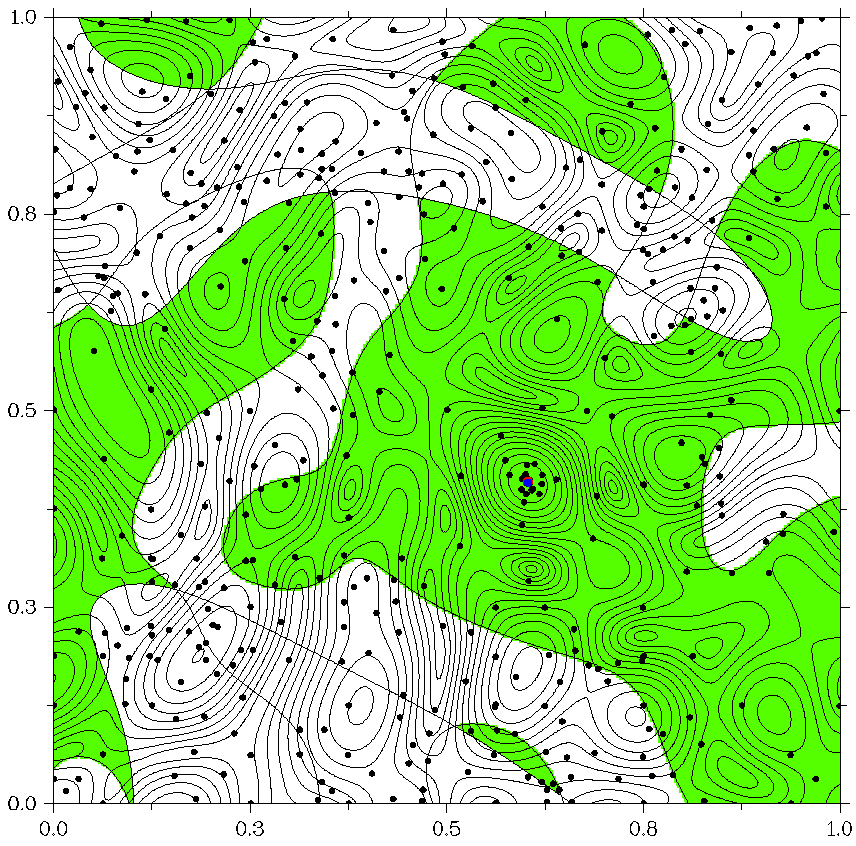
\includegraphics[width=.44\linewidth]{1.png} & 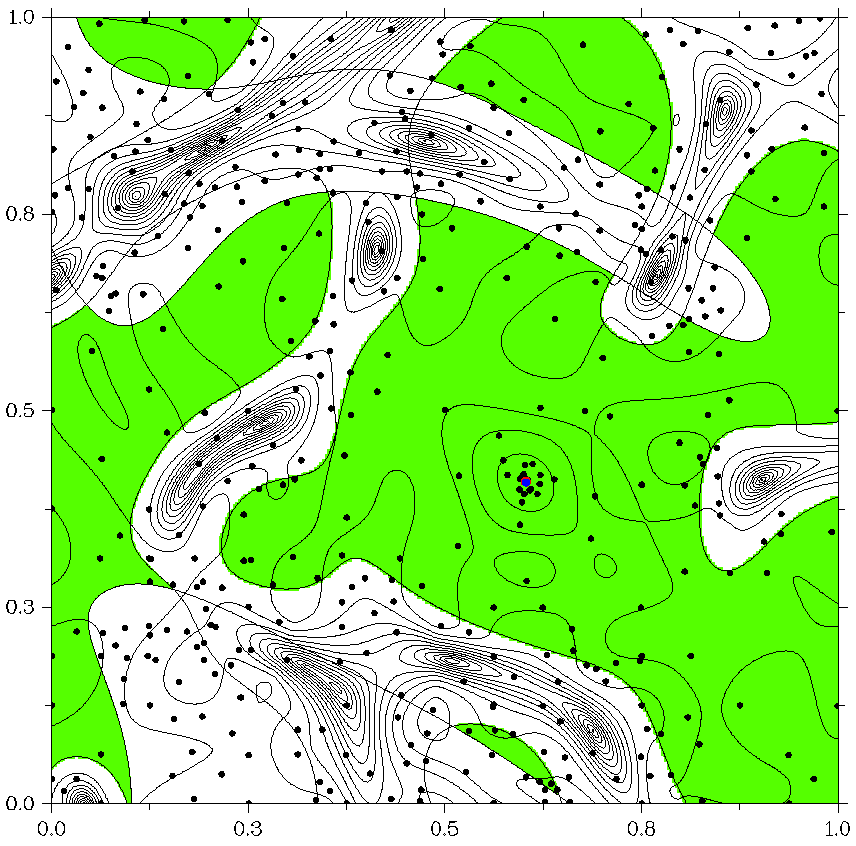
\includegraphics[width=.44\linewidth]{2.png}\\
    \small (a) & \small (b) \\
    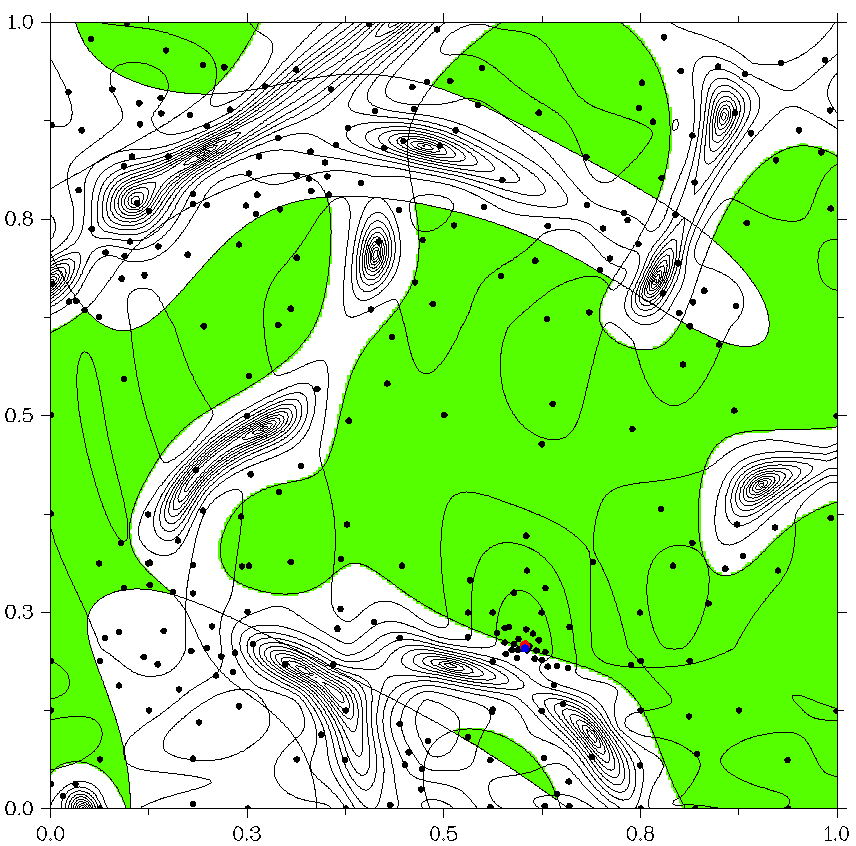
\includegraphics[width=.44\linewidth]{3.png} & 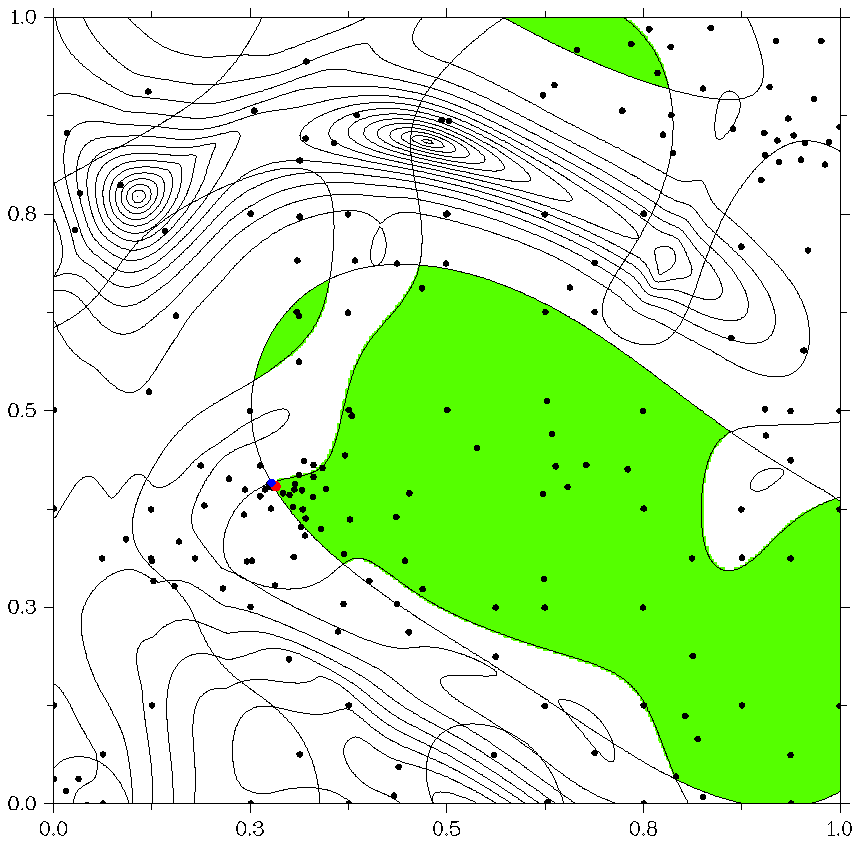
\includegraphics[width=.44\linewidth]{4.png}\\
    \small (c) & \small (d) 
  \end{tabular}
  \caption{The test problems generated by GCGen}
	\label{fig:VAG}
\end{figure}

Fig.~\ref{fig:VAG} (a,b,c,d) also shows the points of 425, 381, 289 and 188 trials, 
correspondingly, performed by the \textit{index method} for solving constrained global 
optimization problems until the required accuracy $\epsilon=10^{-2}$ was achieved. The 
conditional optimizer is shown as a red point and the best estimation of the optimizer is shown 
as a blue point.

The index method has been proposed and developed in 
\cite{Strongin2000,Sergeyev2001,Barkalov2002}. The approach is based on a separate 
accounting for each constraint of the problem and is not related to the use of the penalty 
functions. According to the rules of index method, every iteration includes a sequential 
checking of fulfillment of the problem constraints at this point. The first occurrence of violation 
of any constraint terminates the trial and initiates the transition to the next iteration. This allows: 
(i) accounting for the information on each constraint separately and (ii) solving the problems, in 
which the function values may be undefined out of the feasible domain. 
%It should be noted, that the index method can be efficiently parallelized for accelerators 
%\cite{Barkalov2015,Barkalov2016}.


\section {Conclusion}

This paper considers the method for generating the global optimization test problems with non-
convex constraints, which allows:
\begin{itemize}
	\item controlling the size of the feasible domain with respect to the whole domain of the 
parameters' variation;
	\item knowing a priori the conditional global minimizer of the objective 
function;
	\item generating the unconditional global minimizer of the objective function out of the 
feasible domain;
	\item generating the problems with a conditional minimizer located at the boundary 
of the feasible domain;
	\item defining the number of constraints active at the optimum point.
\end{itemize}

The developed approach allows generating any number of test global optimization problems 
with non-convex constraints for performing computational experiments in order to 
obtain a reliable evaluation of the efficiency of the developed optimization algorithms.

% Acknowledgement
\section{ACKNOWLEDGMENTS}
This research was supported by the Russian Science Foundation, project No 16-11-10150.

% References

%\nocite{*}
\bibliographystyle{aipnum-cp}%
\bibliography{LeGo}%


\end{document}

